\documentclass[10pt,journal,compsoc]{IEEEtran}



% *** CITATION PACKAGES ***
%
\ifCLASSOPTIONcompsoc
  % The IEEE Computer Society needs nocompress option
  % requires cite.sty v4.0 or later (November 2003)
  \usepackage[nocompress]{cite}
\else
  % normal IEEE
  \usepackage{cite}
\fi

% *** GRAPHICS RELATED PACKAGES ***
%
\ifCLASSINFOpdf
 
\else
  
\fi

\ifCLASSOPTIONcompsoc \usepackage[caption=false,font=normalsize,labelfon
t=sf,textfont=sf]{subfig}
\else
\usepackage[caption=false,font=footnotesize]{subfi g}
\fi


\usepackage{graphicx}
\usepackage{algorithmic}
\usepackage{algorithm}
\renewcommand{\algorithmicrequire}{\textbf{Input:}} 
\renewcommand{\algorithmicensure}{\textbf{Output:}}
\usepackage{amsfonts,amssymb}

% \usepackage{cases}
\usepackage{amsmath}
\usepackage[overload]{empheq}
\newcommand{\for}{\text{for }}

\newcommand\MYhyperrefoptions{bookmarks=true,bookmarksnumbered=true,
pdfpagemode={UseOutlines},plainpages=false,pdfpagelabels=true,
colorlinks=true,linkcolor={black},citecolor={black},urlcolor={black},
pdftitle={Bare Demo of IEEEtran.cls for Computer Society Journals},%<!CHANGE!
pdfsubject={Typesetting},%<!CHANGE!
pdfauthor={Michael D. Shell},%<!CHANGE!
pdfkeywords={Computer Society, IEEEtran, journal, LaTeX, paper,
             template}}%<^!CHANGE!

\hyphenation{op-tical net-works semi-conduc-tor}

\begin{document}

\title{Availability-aware Mobile Service Composition Over Oppotunistic Networks}

\author{XX~X,~
		% \IEEEmembership{Student Member,~IEEE,}
		XX~X,~\IEEEmembership{Senior Member,~IEEE,}
        XX~X,~\IEEEmembership{Fellow,~IEEE,}
        % and~Jane~Doe,~\IEEEmembership{Life~Fellow,~IEEE}% <-this % stops a space

% \IEEEcompsocitemizethanks{\IEEEcompsocthanksitem M. Shell was with the Department
% of Electrical and Computer Engineering, Georgia Institute of Technology, Atlanta,
% GA, 30332.\protect\\
% note need leading \protect in front of \\ to get a newline within \thanks as
% \\ is fragile and will error, could use \hfil\break instead.
% E-mail: see http://www.michaelshell.org/contact.html
% \IEEEcompsocthanksitem J. Doe and J. Doe are with Anonymous University.}% <-this % stops a space

%\thanks{Manuscript received April 19, 2005; revised August 26, 2015.}
}



% The paper headers
\markboth{Journal of \LaTeX\ Class Files,~Vol.~66, No.~66, October~2017}%
{Shell \MakeLowercase{\textit{et al.}}: Bare Advanced Demo of IEEEtran.cls for IEEE Computer Society Journals}

\IEEEtitleabstractindextext{%
\begin{abstract}
An opportunistic link between two mobile devices or nodes takes place when they are within communication range of each other. Typically, cyber-physical environments comprise a number of mobile devices that are potentially able to establish opportunistic contacts and serve mobile applications in a cost-effective way.
Opportunistic mobile service computing is a promising paradigm capable of utilizing the pervasive mobile computational resources around users. Mobile users are thus allowed to exploit nearby mobile services to boost their computing power without investment into their own resource pool. 
Nevertheless, various challenges, especially its quality-of-service (QoS) and optimal scheduling, are yet to be addressed. Existing studies and related scheduling strategies consider mobile users to be fully stable and available.
In this paper, instead, we propose a framework named mobile service opportunistic network (MSON) and an availability-aware QoS model for service composition. 
We then formulate the problem into an optimization problem and utilize an improved Krill-Herd algorithm to solve it.
Finally, we carry out a case study based on some well-known scientific workflows and a real-world dataset (the D2D contact traces of MIT Reality dataset and the QoS data of QWS dataset). The comparison implies that our proposed approach outperforms traditional approaches, especially those considering stable and fully available mobille services.

% To evaluate the effectiveness and efficiency of our approach, we obtain experimental performance data through a real-world opportunistic network. The experimental results demonstrate that our approach can obtain superior solutions as compared with current standard composition methods in mobile environments. It can yield near-optimal solutions and has a nearly linear complexity with respect to a problem size.

\end{abstract}

% Note that keywords are not normally used for peerreview papers.
\begin{IEEEkeywords}
Mobile Computing, Mobile opportunistic network, Mobile Service Composition, Service-Oriented Architecture, Service availability.
\end{IEEEkeywords}}


% make the title area
\maketitle



\IEEEdisplaynontitleabstractindextext

\IEEEpeerreviewmaketitle


\ifCLASSOPTIONcompsoc
\IEEEraisesectionheading{\section{Introduction}\label{sec:introduction}}
\else
\section{Introduction}
\label{sec:introduction}
\fi


\IEEEPARstart{R}{ecent years} have witnessed the rapid development of mobile devices (e.g., smartphones, tablets, wearable devices, etc.) and mobile communication. Mobile devices are changing the way people getting the information and the people’s daily lives because they allow you multiple ways of communicating almost anywhere at anytime \cite{satyanarayanan2010mobile}.

The number of mobile devices is still booming and it has already surpassed stationary Internet hosts.
Mobile services are also developed and provided at a significant rate, at the same time, the requirements from mobile users are becoming more demanding, i.e., more complicated applications are needed to be run on mobile devices such as virtual reality applications \cite{bastug2017toward} or machine learning applications on mobile phones \cite{abadi2016tensorflow} on mobile phones. However, because of the limited hardware resources of mobile devices (e.g., computational resource, battery life, memory, and storage), these resources-intensive tasks are usually offloaded to mobile computing cloud \cite{dinh2013survey}, which result in high data transfer costs (energy cost and communication fee) and high latency.

\begin{figure}[!t]
\centering
\includegraphics[width=3.5in]{./img/pic1.pdf}
\caption{Opportunistic computing}
\label{Opportunistic computing}
\end{figure}

Opportunistic computing is promising complementary to conventional mobile cloud computing. As illustrated in Fig.1, the basic idea of opportunistic computing is to allow the users to utilize the resources and services that other users share, by exploiting the direct physical contacts between the users, and the resulting potential to exchange data through a direct connection between their devices (e.g. through wireless connection or Bluetooth). Resources and services available on mobile devices can be directly shared among users in a elastic and on-demand way without time-consuming and energy-requiring interactions with pre-existing infrastructure, either at the networking level (e.g., cellular networks) or at the computing/service level (e.g., the cloud). 
Note that, mobile tasks usually require huge computational resources or data transfer (e.g., Tensorflow on mobile, Photoshop on mobile, Online video). Nearby mobile service provider are thus more adept, in terms of energy-efficiency, at executing these tasks than the online services or nodes with the help of device
to device (D2D) communications such as Bluetooth, WiFi and NFC \cite{balani2007energy}. D2D communications are featured by extensively-reduced data transfer delays and required energy than traditional cellular network. Thus it provides better user-perceived service quality in terms of reduced waiting time and improved service responsiveness. It is promising to replenish traditional cellular communications in terms of user throughput increase, cellular traffic reduction and network coverage extension. 

However, due to the change of application environment and application object, service computing in mobile environment faces two inherent challenges.

1) Constant Mobility: Mobile users change their locations frequently, which results in the variation of service availability. Thus, determining how to handle user mobility is a major challenge for providing reliable mobile services in highly dynamic mobile wireless environments.

2) Limited Resource: Mobile devices have limited computing capability compare with other stationary computing devices. But mobile service composition plan must be generated as fast as possible because the availability of mobile service may vary much within a short time. Therefore, composition algorithm must have fast convergence rate and good scalability.

To address the aforementioned challenges and concerns, we propose an availability-aware mobile service composition approach in this paper, where a mobile user in mobile service opportunistic network are allowed to combine and exploit, through D2D communications, nearby devices' resources with time-varying availability (in contrast, traditional approaches mainly consider fully-available mobile services) to boost their computing power and therefore overcome the limitations of their own resources \cite{giordano2011human}. 

The main contributions are:

1) We propose a framework (mobile service opportunistic network, MSON in short) to address the problem of service provisioning in the mobile encounter environment where both service requesters and providers are nonstationary and with time-varying availability. In such environment, mobile user can invoke services exposed by nearby mobile devices through D2D links.

2) For MSON, we propose a availability-aware QoS model for service provisioning to capture users' mobility behavior.

3) Based on MSON and the proposed mobile service QoS model, we formulate the mobile service composition problem to an optimization problem and propose a Krill-Herd based algorithm to solve it. 

% A series of evaluations have been conduct to validate the optimality and scalability of our algorithm, and it shows our algorithm can get approximately optimal solution and better performance than other standard composition approaches. 

% The remainder of this paper is structured as follows. Section II describe the MSON framework and its application scenario. Section III introduces the mobile service composition model. The approach to make service compositions is presented in Section IV. Section V presents experiments and evaluations. Section VI reviews the related work. Section VI concludes this paper.

\section{RELATED WORK}
% Service-oriented computing (SOC) is a novel paradigm to develop and integrate enterprise information system \cite{papazoglou2003service}, with the development of mobile device and communication technology, the research of mobile service composition has grain much attention from both industry and academia. In this section, we first briefly review some recent work on mobile service composition, then review opportunistic network and its application in mobile devices.

\subsection{mobile service composition}
Mobile service composition refers to the technique of creating composite services with the help of smaller, simpler and easily executable services or components over mobile networks. Recent technological advances in novel mobile device design and development as well as wireless networking materialize a vision where devices all around a user, either embedded as a part of smart spaces, or being carried by other users
near by, are enabled to present services probably useful. Users sometimes look for services that are not pre-existent on any device but can be dynamically built by appropriately combining already existing ones. For this purpose, extensive research efforts are carried out in this direction. For example, Deng et al. \cite{Deng2016} classify mobile service composition methods into three categories: C2M, M2M, Hybrid. They also discussed the challenge toward mobile service provisioning and mobile service composition in terms of performance, energy and security perspective. They also proposed a mobile-service-sharing-community model and extend the random way point (RWP) model to capture user mobility. They utilize the meta-heuristic algorithm to decide the optimal compositional plan. Yang et al. \cite{Yang2010} present a comprehensive QoS model specifically for pervasive services. They consider not only mobile wireless network characteristics but also user-perceived factors. They derive a corresponding formula to calculate the QoS criterion. 
zhang et al. \cite{Zhang2016qos} consider a context-aware service selection algorithm based on Genetic Algorithm, They introduce a tree-encoding method to improve the capacity and efficiency of GA. However, for simplicity of the proposed model, they do not consider user mobility.
Wang et al. \cite{wang2011exploiting} model dependable service composition in wireless mobile ad hoc networks by considering mobility prediction of the service providers.
They use a probability-free model and a probabilistic model to characterize the uncertainty of composing. A service that can tolerate a certain level of the mobility of service providers. However, for simplicity of their proposed model, they focus on only the workflows. Besides, the heuristic algorithms they presented fails to decide the optimal compositional plan.

\subsection{mobile opportunistic network}
Opportunistic networking is one of the most promising evolutions of the traditional multi-hop networking. Instead of relying itself on stable end-to-end paths as in the Internet, opportunistic networks do not consider node mobility a problem but as an useful opportunity. 
Marco et al. \cite{Conti2014} give a review of opportunistic network and regarded it as the first step in people-centric networking, they also discuss the focused research problem such as mobility model and routing problem.
Turkes et al. \cite{turkes2016cocoon} proposed a middleware named Cocoon to support mobile opportunistic network, they design a routing protocol above Wi-Fi and Bluetooth standards, their experiments which use real-world data setups show that Cocoon performs well on the aspects of dissemination rate, delivery latency and energy consumption.
Fortuna et al. \cite{fortuna2009dynamic} presented an review of dynamic service composition over both wired and wireless environment, However, their work does not present any technical details to describe how to composite service in mobile networks.
Giordano et al. \cite{giordano2011human} proposed a novel paradigm that utilize Opportunistic computing as an appealing complement to the mobile computing cloud, in this way, mobile device can combine and exploit heterogeneous resources from other devices.
Pu et al. \cite{Pu2017crowd} presented QoS-oriented self-organized mobile crowdsourcing framework, in this work, the prevalent and sufficient characteristics of opportunistic user encounters in our daily life are utilized to solve crowdsourcing problem.


\section{mobile service opportunistic network}

\begin{figure}[!t]
\centering
\includegraphics[width=3.5in]{./img/pic2.pdf}
\caption{Mobile service opportunistic network}
\label{fig_mson}
\end{figure}

In this section, we first introduce the characteristics of mobile service opportunistic network (MSON), then a user case is presented to illustrate its application scenario, it is also assumed that MSON has the following properties:

1) Locality: Rather than stable internet, an MSON bases itself on mobile networks and exploits user mobility. Mobile users in MSON can perceive nearby services and establish self-organized local communication within permitted transmission distance.

2) Mobility: Service requesters and providers keep moving in the mobile network even when they are invoking or provisioning mobile services.

3) Nondeterminism: Mobile services shared in an MSON are transient because the relative distance between any two services keeps changing and could rise above the permitted transmission distance at any time. 

Fig. 2 illustrates how the mobile services provision over MSON. In an MSON, a mobile service requester can perceive mobile services exposed by nearby devices through D2D links and launch a request for mobile service composition. A composer process, which is in charge of discovering available mobile services nearby, selecting appropriate concrete services, and composing selected services. All concrete services interact with the composer directly \cite{Deng2017}.

Note that, we consider only one-hop D2D links for both service requesters and providers. 
Because D2D communications which hops are larger than two would incur network overhead \cite{li2014can} while one-hope communications can lower the delay (e.g., no need to transfer a large volume of task contents hop by hop) and ensure framework choose only local relatively reliable service. 
Besides, some existing researches \cite{chang2015progressive,tuncay2013participant,wu2013homing,jiang2016exploiting,liu2013exploring} reveal that users' one-hop neighbors are sufficient enough, compared with multi-hop mechanisms.

We use an simple user case to illustrate the related features of service provision over MSON. 
Consider a mobile user who is in a crowded subway and his mobile phone has low battery. 
Now he wants to edit some videos, add some effects and share these video clips to his friends. 
If he do all these operations on his own mobile phone, his mobile phone will run out of energy because of limited battery. 
As one option, he can upload original videos to cloud and use cloud service to get all things done, but offloading task into cloud will result in heavy cellular traffic, which means high energy consumption and expensive communication fee.
But if he is a participate in MSON and several video processing services is provided by some nearby mobile devices, he can invoke such mobile services on nearby mobile devices through D2D communications. 
If these services cannot meet his requirement, several services can be composed. 
Due to users' mobility, the availability of service can vary, invoking mobile services provided by other users may face new challenges that traditional composition methods cannot handle. 
Thus, a mobile service composition model which can capture mobile services' availability need to be proposed.

\section{MOBILE SERVICE COMPOSITION MODEL}
\subsection{Preliminaries}
To facilitate modeling, reasoning, and analysis of the mobile service composition problem, we first present some basic definitions.

\textit{Definition 1 (Mobile Service):} A mobile service is denoted by a two-tuple $ms = (info, QoS)$, where:

1) $info$ is the description of a mobile service which include service name, functionality, input parameters and response data.

​2) $QoS = \{ q_{rt}, q_{price}, q_{ava}, ... \}$ is a set of quality attributes, including response time, price, availability, etc.

\textit{Definition 2 (MSON participant):} A MSON participant is mobile service user who can be a service provider or a requesters. It is denoted by a two-tuple $u = (P, C)$, where:

​1) $P$ is the set of mobile services exposed to other MSON participants.

​2) $C$ is the set of mobile services discovered from nearby MSON participants.

\textit{Definition 3 (Mobile Service Composition Plan):} A Mobile Service Composition Plan $mscp = (T, E)$ is modeled as a directed acyclic graph (DAG) where $T = {t_1, t_2, ..., t_n}$ is the set of tasks and $E$ is the set of directed edges. An edge $e_{ij}$ of the form $(t_i,t_j)$ exists if there is a data dependency between $t_i$
and $t_j$, case in which $t_i$ is said to be the parent task of $t_j$ and $t_j$ is said to be the child task of $t_j$. Based on this definition, a child task cannot be executed until all of its parent tasks are completed.

\subsection{Mobile Service Availability}
\begin{figure}[!t]
\centering
\includegraphics[width=3in]{./img/pic3.pdf}
\caption{Mobile service availability}
\label{fig_sd}
\end{figure}
In an MSON, the availability of mobile service is variable and dynamically by users' mobility. 
As illustrated by an example in Fig. 3, there are two mobile users $i$ and $j$ with identical transmission rage R. User $i$ is a mobile service requester while user $j$ a mobile service provider. Each user moves freely and it is assumed that the moving area is a circle with a radius of $r$ in a certain amount of time. $d$ is the distance between $i$ and $j$. If user $j$ moves outside the transmission range of its neighbouring user $i$, then user $j$ is unreachable for user $i$ and consequently the services on user $j$ become unavailable to user $i$ \cite{Yang2010}.

Suppose a mobile service running on mobile node $j$ is a candidate service for a task requested by user $i$, and the availability of candidate service (denote as $Ava(i,j)$) equals the probability of user $j$ staying inside the transmission range of user $i$, and it can be calculated as follow: 
\begin{equation}
Ava(i,j) = \frac{S_{i \bigcap j}}{S_j}
\end{equation}
Where $S_{i \bigcap j}$ is the area of the user $j$ moving field inside the transmission range of user $i$, $S_j$ is the moving field area of the user $j$.

We use $r$, $R$ and $d$ to calculate $S_{i \bigcap j}$ and $S_j$. 
The transmission range of a node $R$ is a preset value (e.g., usually 10m for bluetooth and 25m for Wi-Fi). 
Note that most of wireless transaction protocols have defined the RSSI (Received Signal Strength Indicator), then distance $d$ between mobile user $i$ and user $j$ can be calculated by signal strength.  
The moving radius of a mobile user $r$ is its moving speed $v$ multiplied by the average service time $t$. Here $t$ can be statistically calculated as the average value of last $n$ times of service invoke, namely, $t = \Sigma_{i=1}^{n}t_i/n$. The speed of a mobile user $v$ can be get through GPS data or other mobile sensor (e.g., Gyro-sensor), then $r = v \times t$. ​

Finally, $S_{i \bigcap j}$ can be calculated as follow:
\setlength{\arraycolsep}{0.0em}
\begin{align}
S_{i \bigcap j} & =  [(\frac{2\alpha}{2\pi} \times \pi r^2)-(\frac{r sin\alpha cos\alpha}{2} \times 2)]\\\nonumber
& \ \ \ \ +[(\frac{2\beta}{2\pi} \times \pi R^2)-(\frac{R sin\beta cos\beta}{2} \times 2)]\\\nonumber
& = \alpha r^2 + \beta R^2 - (r^2 sin\alpha cos\alpha + R^2 sin\beta cos\beta)
\end{align}
\setlength{\arraycolsep}{5pt}
Where
\begin{eqnarray}
\alpha = arccos(\frac{r^2+d^2-R^2}{2r\times d}) \\\nonumber
\beta = arccos(\frac{R^2+d^2-r^2}{2R\times d})
\end{eqnarray}

$S_j$ can be calculated by:
\begin{align}
S_j & = \pi r^2 \\\nonumber
& = \pi \times (s \times t)^2
\end{align}

Therefore, the availability of mobile service between requester $i$ and provider $j$ in a certain time can be calculated as follow:
\begin{align}
Ava(i,j) = \frac{\alpha r^2 + \beta R^2 - (r^2 sin\alpha cos\alpha + R^2 sin\beta cos\beta)}{\pi s^2 t^2}
\end{align}
Mobile service availability can capture user's mobile behavior, and we use it as an important QoS attribute to construct QoS model for service composition in next subsection.

\subsection{QoS Model for Mobile Service Composition}
For mobile service requesters to select candidate service, QoS must be considered \cite{Wu2016,luo2014efficient,luo2016generating}. Generally, QoS attributes include response time, price, reliability, and reputation, we introduce mobile service availability as an important QoS attribute in this paper to describe user's mobility behavior. QoS attributes in this paper can be classified into two categories: positive ($Q^+$) and negative ($Q^{-}$). For positive attributes, larger values indicate better performance (e.g., reputation and availability), while for negative attributes, smaller values indicate better performance (e.g., response time and cost).

\begin{table}[!t]
\renewcommand{\arraystretch}{1.3}
\caption{Examples of aggregation functions for QoS}
\label{aggregation functions}
\centering
\begin{tabular}{ccc}
\hline
\bfseries Pattern & \bfseries Resopnse Time & \bfseries Availability \\
\hline
sequence & $\sum_{i=1}^{n}q_{rt}(S_i)$ & $\prod_{i=1}^{n}q_{ava}(S_i)$ \\
parallel & $Max\{q_{rt}(S_i)\}$ & $\prod_{i=1}^{n}q_{ava}(S_i)$ \\
choice & $\sum_{j=1}^{n} p_j \times q_{rt}(S_j)$ & $\sum_{j=1}^{n} p_j \times q_{ava}(S_j)$ \\
loop & $k \times q_{rt}(S_i)$ & $[q_{ava}(S_i)]^{k}$ \\
\hline
\end{tabular}
\end{table}

A service composition instance $csi$ can be represented as $csi = \{s_{(1,i)}, s_{(2,j)},...,s_{(n,k)}\}$, where $s_{(j,k)}$ is the selected concrete services. For example, $s_{(1,i)}$ means the $i$-th service candidate is selected to execute $task_1$. For a $csi$, its each QoS attribute is determined by its concrete components and orchestration patterns. Table.1 lists the aggregation functions for response time and availability for sequential, loop, choice, and parallel composition patterns. We can find more aggregation functions found in \cite{jaeger2004qos} and \cite{zheng2013qos}.

In order to facilitate ranking of different composite service instances $csi$ in terms of QoS, we utilize simple additive weighting (SAW) as the QoS utility function to map the QoS value into a real value. SAW first normalizes the QoS attribute values into real values between $0$ and $1$, through comparison with the maximal and minimal values; then it sums the normalized values multiplied with a preference weight $w_t$. According to SAW, the QoS utility of a $csi$ can be calculated using e.q (6), where, $q_t(csi)$ is the aggregated value of the type-$t$ QoS attribute of $csi$, and $q_{t,max}$ and $q_{t,min}$, respectively, denote the maximal and minimal possible aggregated values of the type-$t$ QoS attribute \cite{Wu2016}.
\begin{align}
U(csi) = & \sum_{q_t \in Q^-} \frac{q_{t,max}-q_t(csi)}{q_{t,max}-q_{t,min}}\times w_t \\\nonumber
& +\sum_{q_t \in Q^+} \frac{q_t(csi)-q_{t,min}}{q_{t,max}-q_{t,min}}\times w_t
\end{align}

\subsection{Problem Formulation}
Base on the above discussion, we can give the definition of the service composition over MSON problem.

\textit{Definition 4 (MSON Service Composition):} Given a service composition request $req$ by a mobile user $u$, perceive nearby service and select suitable concrete services to achieve an optimal service composition instance $csi$ with the best QoS, that is
\begin{align}
maximize      \ \ : \ \ & U(csi)   \\\nonumber
subject\ to   \ \ : \ \ & t_i \in \{1,2,3,...,n\}  \\\nonumber
                        & s_i \in \{1,2,3,...,m \}
\end{align}
where $U(csi)$ is the objective function mentioned in e.q (6), $t_i \in [1,n]$ is the index of the tasks in the composition plan, $s_i \in [1, m]$ is the index of service candidates for the $i$-th task.

\textit{Theorem 1:} The service composition problem over MSON (Definition 6) is NP-hard.

\textit{Proof:} We can reduce the service composition problem over MSON problem to a knapsack problem, and this problem can be solved by integer programming. 
The canonical form of integer linear program to search the optimal solution of this problem can be expressed as follow \cite{papadimitriou1998combinatorial}:\
\begin{align}
maximize     \ \ : \ \ & F(X) = c^{T}X     \\\nonumber
subject\ to  \ \ : \ \ & Ax \le b, \\\nonumber
               	       & x_i \in \mathbb{Z}^{n} \\\nonumber
                       & x_i > 0 
\end{align}
Where $F(x)$ is objective function, $X$ is feasible solution, $n$ is a positive integer, $b$ and $c$ are vectors, $A$ is a matrix.
%matrix $A$ and vector $b$ construct the constrain of service candidates bounds, vector $c$ means how to map the feasible solution $x$ to objective value.
For the problem of selecting optimal services composition over MSON, the vector $X = \{s_{(1,i)}, s_{(2,j)}. . . , s_{(n,k)}\}$ can describe a feasible solution as a service composition with $n$ tasks. 
% An element $ms_{1i}$ in corresponds to a selected service from the candidates for the $1$-th task.
The optimal solution  $X^*$ satisfies the following conditions:

1) $X^*$ is a feasible solution.

​2) for all feasible $X$, $F(X^*) \le F(X)$. 

The target of the mobile service composition problem over MSON is to find the biggest $F(x)$. Thus, the problem is equivalent to the integer programming problem which is known to be NP-hard. Then the service composition problem over MSON is NP-hard.

\section{The kh-based algorithm for mobile service composition}
For the problem we formulate above, integer programming can be utilized to obtain the optimal solution. However, integer programming might cost much more time with the increment of problem size because of its poor scalability \cite{nemhauser1988integer}. To solve this problem in polynomial time, an meta-heuristic algorithms such as GAs and PSO, can be utilized to find the near optimal solution.
%In this section, we will illustrate our algorithm for making mobile service compositions over MSON based on the Krill-Herd algorithm.

Krill-Herd algorithm \cite{gandomi2012krill} is new generic stochastic optimization approach for the global optimization problem which is inspired by predatory behavior and communication behavior of krill. 
% The whole process of the IKH algorithm is shown as fig.4.
In this section, we will introduce a Krill-Herd based algorithm to solve the problem of mobile service composition over MSON.

% \begin{figure}[!t]
% \centering
% \includegraphics[width=3in]{./img/pic6.pdf}
% \caption{KH algorithm}
% \label{fig_opportunistic}
% \end{figure}

\subsection{Encoding}
%In this paper, the position vector of each krill individual corresponds to a feasible mobile service composition,
In KH, composite service instance is encoded as a krill individual, the krill individual with the best position corresponds to the optimal mobile service composition. The target of algorithm is to find the krill individual with the best position, which means to find the best mobile service composition with the best QoS utility. Therefore, once the optimal krill individual is found, the best mobile service composition is obtained.

In this paper, the position vector of each krill individual is represented by an integer array with its length equal to the number of involved tasks. The $i$-th entry in the array, in turn, refers to the selection result of the task $t_i$ . That is to say, given that the value of the $n$-th entry is $k$, it indicates that $s_{(n,k)}$ is the selected concrete service to execute $t_n$. Fig. 4 illustrates this krill encoding.

\begin{figure}[!t]
\centering
\includegraphics[width=3in]{./img/pic4.pdf}
\caption{Krill encoding}
\label{Krill encoding}
\end{figure}


\subsection{Motion operator}
% 
% 

Motion operator is the key component of KH algorithm. As shown in e.q (10), the position of each krill individual is determined by three main factors: 1) motion influenced by other krill; 2) foraging action; 3) physical diffusion. 
\begin{equation}
\frac{dX_i}{dt} =N_i+F_i+D_i
\end{equation}

where individual $X_i = \{ms_{(1,j)}, ms_{(2,k)}, . . . , ms_{(n,l)}\}$ represents the $i$-th composition service instance in population, $n$ is the number of tasks in the service composition, $N_i$, $F_i$, and $D_i$ denote the motion influenced by other krill individuals, the foraging motion, and the physical diffusion, respectively.

1) Movement induced by other krill individuals

The motion induced by other krill individuals $N_i$ means to learn from neighbor mobile service compositions. It can be formulated as follow:
\begin{equation}
N^{new}_i = N_{max}\alpha_i + \omega_n N^{old}_i
\end{equation}

where
\begin{equation}
\alpha_i = \alpha^{target} + \alpha^{local}
\end{equation}

$\alpha_i$ is the direction of the induced motion and it can be evaluated by target swarm density (target effect $\alpha^{target}$), local swarm density (local effect $\alpha^{local}$). $N_{max}$ is the maximum induced speed, $\omega_n \in [0, 1]$ the inertia weight of the induced motion, $N^{old}_{i}$ is the last induced motion influenced by other krill individuals.

2) Foraging Motion

Similarly, the foraging motion $F_i$ is to learn from the current optimal composite service instance. 
$F_i$ has two parts: the current food location and the information about the previous location. 
For the individual $X_i$, we can formulate this motion as follow
\begin{equation}
F_i = V_f\beta_i + \omega_f F^{old}_i
\end{equation}
where
\begin{equation}
\beta_i = \beta_i^{food}+\beta_i^{best}
\end{equation}
where $V_f$ is the foraging speed, $\omega_f \in [0, 1]$ is the inertia weight of foraging, and $F^{old}_i$ is the last foraging motion. $\beta_i$ is the direction of the foraging motion.

3) Random diffusion

For individual $X_i$, the physical diffusion is considered to be a random process. This motion includes two components: a maximum diffusion speed and a random directional vector, it can be formulated as follow

\begin{equation}
D_i = D_{max}\delta
\end{equation}

where $D_{max}$ is the maximum diffusion speed and $\delta \in [-1, 1]$ is a random directional vector.

\subsection{Stud selection and crossover operator}

\begin{figure}[!t]
\centering
\includegraphics[width=2.5in]{./img/pic5.pdf}
\caption{Crossover operator}
\label{Crossover operator}
\end{figure}


The crossover operator plays an important role in Genetic algorithm for global optimization, we use this operator in KH algorithm to enhance the search capability. The crossover operator in this paper is controlled by a dynamic crossover rate $C_{rate}$ which can be obtain as follow
\begin{equation}
C_{rate} = Cr + (1-Cr) \times \frac{U_{best}-U_{i}}{U_{best}-U_{worst}}
\end{equation}

Where $C_r$ is a pre-set fixed crossover rate, $U_{i}$ is the $i$-th individual's QoS utility, $U_{best}$ is the current best QoS utility value, similarly, $U_{worst}$ is the current worst QoS utility value. 

Then we can use $C_{rate}$ to generate $i$-th individual's crossover vector $Cv = \{c_{1},c_{2},...,c_{n}\}$, it can be manipulated as follows

\begin{equation}
c_{i}=
\begin{cases}
1,& if \ \ rand(0,1) < C_{rate}\\
0,& else\\
\end{cases}
\end{equation}

Inspired by SGA \cite{khatib1998stud} (a type of GA which employs the optimal genome for crossover at each generation), we introduce stud selection procedure to improve KH's search capability.
From algorithm 1, we can see that for each individual $X_i$ to crossover, we choose the optimal individual $Stud$ (i.e., the individual with highest QoS utility value) to mating. As shown in Fig. 5, the characteristics from individual $Stud$ are copied to individual $X_i$ according to crossover vector $Cv$. 

\begin{algorithm}
\caption{Crossover operation}
\label{alg1}
\begin{algorithmic}[1]

\REQUIRE Population $X$; Individual $X_i$ to crossover; The number of tasks $taskNumber$; 
\STATE Sort all krill individuals in population $X$ by its QoS utility, get optimal individual $Stud$, save the best QoS utility value as $U_{best}$ and the worst QoS utility value as $U_{worst}$
\STATE $C_{rate} \leftarrow$ calcCrossoverRate($X_i$, $U_{best}$, $U_{worst}$)
\FOR{$i=0$ \TO $taskNumber$}
\STATE $r \leftarrow rand(0,1)$
\IF{$r < C_{rate}$}
\STATE $Cv[i] \leftarrow 1$
\ELSE
\STATE $Cv[i] \leftarrow 0$
\ENDIF
\ENDFOR
\FOR{$i=0$ \TO $taskNumber$}
\STATE $X_i[i] \leftarrow X_i \wedge  (1-Cv[i]) + Stud \wedge Cv[i]$ 
\ENDFOR
\end{algorithmic}
\end{algorithm}

\subsection{Update position}
After crossover, the offspring should be evaluated and updated to current evolutionary sequence.
According to the three motion actions, the time-relied position from time $t$ and $\Delta t$ can be formulated by the following equation
\begin{equation}
X_{i+1} = X_i + \Delta t \frac{dX_i}{dt}
\end{equation}

where
\begin{equation}
\Delta t = C_t\sum_{j=1}^{n}(UB_j - LB_j)
\end{equation}

where $n$ is the tasks number of composition service, $UB_j$ and $LB_j$ are upper and lower bounds of candidate services for the $j$-th task, respectively. $C_t$ is a constant value to scale the searching space and we set it to $1/2n$ in this paper. Finally, the overall KH algorithm process can be describe in Algorithm 2.

\begin{algorithm}
\caption{KH algorithm}
\label{alg2}
\begin{algorithmic}[1]

\REQUIRE Number of population size $PS$, Number of max iteration $MI$;

\STATE Generate initial population as $X = (X_1, X_2, ..., X_{PS})$
\STATE Evaluate the QoS utility value of each krill individual in $X$
\FOR{$i=0$ \TO $MI$}
	\FOR{$i=0$ \TO $PS$}
		\STATE $X_i^{'} \leftarrow motionOperator()$
		\STATE $X_i^{''} \leftarrow crossoverOperator(X_i^{'})$
		\STATE $U_i^{'} \leftarrow evaluateQoSutility(X_i^{'})$
		\STATE $U_i^{''} \leftarrow evaluateQoSutility(X_i^{''})$
		\IF{$U_i^{''} < U_i^{'}$}
			\STATE update position by equation (18) as $X_{i+1}$
		\ELSE
			\STATE accept $X_i^{''}$ as $X_{i+1}$
		\ENDIF
	\ENDFOR
\ENDFOR
\STATE Output the best solution
\end{algorithmic}
\end{algorithm}

\section{SIMULATION AND EVALUATION}
In this section, we first discussed the experimental environment settings, and then the KH-based approach for the mobile service composition algorithm is evaluated from the perspective of optimality and scalability, respectively.
\subsection{Simulation Setting}
To evaluate the optimality and scalability of the proposed approaches, the experiment is run on a personal computer with an Intel Core i5 CPU with 2.4 GHz, 4 GB RAM, macOS and Matlab R2015b Edition.

Since we can not find available realistic datasets which involving both user D2D contact traces and quality of mobile service so far, we attempt to simulate the scenarios for mobile services provision by integrating realistic user D2D contact traces with quality of Web service datasets. 

We consider MIT Reality dataset \cite{eagle2006reality} as user D2D contact traces, where user location, Bluetooth devices in proximity, application usage, and phone status (such as charging and idle) were collected from 100 users over several months. This dataset can really reflect diverse network scenarios.

The publicly available quality of Web service (QWS) dataset\cite{zheng2014investigating} can be used to characterize the service candidates. This dataset consists of 4500 Web services from 142 users over 64 different time slices (at 15-minute interval) and each QoS data includes two measurements (response time and throughput).
% for a mobile service, response time attribute is randomly selected from the QWS dataset. 

\begin{table}[!t]
\renewcommand{\arraystretch}{1.5}
\caption{User $u$ 's D2D contract traces}
\label{D2D contract traces}
\centering
\begin{tabular}{c c}
\hline
\bfseries Time & \bfseries Available service provider\\
% user(3).devices_names(500-505)
% \hline
\hline
t1 & Rabbit, Tony, S10, BlueRadios, NORTHOLT\\
% \hline
t2 & Tony, S10, Rabbit, NORTHOLT, BlueRadios\\
% \hline
t3 & Rabbit, NORTHOLT, BlueRadios, S10, Tony, Henrymobile, S4 \\
% \hline
t4 & Tony, NORTHOLT, BlueRadios, S10, Rabbit, S4\\
% \hline
t5 & BlueRadios, S4, AliKatz, NORTHOLT, Rabbit, S25, S10\\
% \hline
t6 & S25, S10, NORTHOLT, BlueRadios, Rabbit\\
% \hline
... & ...\\
\hline
\end{tabular}
\end{table}

\begin{table}[!t]
\renewcommand{\arraystretch}{1.3}
\caption{Services exposed by provider}
\label{Services exposed by provider}
\centering
\begin{tabular}{c c}
\hline
\bfseries Service Provider & \bfseries Exposed Service\\
% user(3).devices_names(500-505)
\hline
% \hline
AliKatz     & $ms_1$, $ms_2$, $ms_3$, $ms_4$\\
% \hline 
BlueRadios  & $ms_1$, $ms_5$\\
% \hline
Henrymobile & $ms_2$, $ms_4$\\
% \hline
NORTHOLT    & $ms_4$, $ms_5$, $ms_6$ \\
% \hline
Rabbit      & $ms_1$, $ms_4$\\
% \hline 
S4          & $ms_1$, $ms_2$\\
% \hline 
S10         & $ms_6$, $ms_7$\\
% \hline 
S25         & $ms_4$, $ms_5$\\
% \hline 
Tony        & $ms_1$, $ms_4$\\
% \hline 
... & ...\\
\hline
\end{tabular}
\end{table}

\begin{table}[!t]
\renewcommand{\arraystretch}{1.8}
\caption{Available candidates}
\label{Available candidates}
\centering
\begin{tabular}{c c}
\hline
\bfseries Time & \bfseries Available service\\
% user(3).devices_names(500-505)
\hline
% \hline
t1     & $ms_1^{(3)}$, $ms_4^{(3)}$, $ms_5^{(2)}$, $ms_6^{(1)}$, $ms_7^{(1)}$ \\
% \hline 
t2     & $ms_1^{(3)}$, $ms_4^{(3)}$, $ms_5^{(2)}$, $ms_6^{(2)}$, $ms_7^{(1)}$ \\
% \hline
t2     & $ms_1^{(4)}$, $ms_2^{(2)}$, $ms_4^{(4)}$, $ms_5^{(2)}$, $ms_6^{(2)}$, $ms_7^{(1)}$ \\
% \hline
t4     & $ms_1^{(4)}$, $ms_2^{(1)}$, $ms_4^{(3)}$, $ms_5^{(2)}$, $ms_6^{(2)}$, $ms_7^{(1)}$ \\
% \hline
t5     & $ms_1^{(4)}$, $ms_2^{(2)}$, $ms_3^{(1)}$, $ms_4^{(4)}$, $ms_5^{(3)}$, $ms_6^{(2)}$, $ms_7^{(1)}$ \\
% \hline 
t6     & $ms_1^{(2)}$, $ms_4^{(3)}$, $ms_5^{(3)}$, $ms_6^{(2)}$, $ms_7^{(1)}$ \\
% \hline 
... & ...\\
\hline
\end{tabular}
\end{table}

Table 2 is part of D2D contract traces in MIT Reality dataset. For example, there there are five nearby devices within D2D transmission distance at time $t1$ and these devices can be regarded as MSON participant who provision mobile services. Table 3 shows MSON participants and the services they exposed to nearby devices. These mobile service are random chosen from QWS dataset. Table 4 is the Cartesian product of Table 2 and Table 3, it shows how many kinds of services user can exploit at a certain time and how many candidates for each kind of service (i.e., task). For example, there are five kinds of service available at time $t1$ and there are three candidates for task $t_1$, three candidates for task $t_4$, two candidates for task $t_5$, one candidate for task $t_6$ and one candidate for task $t_7$.

\subsection{Impact of Parameters}
There are six parameters can be adjusted to improve the IKH's performance: population size $PS$, maximum iteration number $MI$, crossover rate $Cr$, foraging speed $V_f$, maximum induced speed $N_{max}$ and physical diffusion speed $D_{max}$. As shown in Table 5, we generate six groups of parameters configuration to evaluate the impact of each parameter. For each group of parameters configuration, we tune one parameter and fix the other parameters. For each configuration setting, the IKH algorithm is executed 50 times independently and the average performance was recorded.

%    KH_profile.NK         = 20;
%    KH_profile.MI         = 30;
%    KH_profile.CR         = 0.6;
%    KH_profile.Vf         = 0.8;
%    KH_profile.Nmax       = 0.3;
%    KH_profile.Dmax       = 0.2;
Fig. 5(a) shows the impact of population size, we observe that with the increase of population size, the average QoS utility of IKH significantly improved before $PS=10$, and no significant improvement is observed after population size over $20$. Therefore, an excessively large population size (e.g., $PS=50$) has limited impact on the performance of IKH, and it will result in computing resources waste and high time cost.
Similarly, Fig. 5(b) shows that the value of QoS utility significantly increased for higher number of iteration times until to a limit: $MI = 30$. 
Fig. 5(c) shows the impact of the crossover rate $Cr$. The performance of KH increases with $Cr$ firstly, then decrease, the best performance is achieved for $Cr = 0.6$.
Fig. 5(d) shows the impact of the foraging speed $V_f$. The performance of IKH increases with $V_f$ firstly, then decrease, the best performance is achieved for $V_f = 0.8$.
Fig. 5(e) shows the impact of the induced speed $N_{max}$. The performance of IKH increases with $N_{max}$ firstly, then decrease, the best performance is achieved for $N_{max} = 0.3$.
Fig. 5(f) shows the impact of the physical diffusion speed $D_{max}$. It shows that with the increase of $D_{max}$ the performance of IKH fluctuation irregularly and slightly, without loss of generality, we random generate $D_{max}$ from $[0.2 \sim 0.5]$ in this paper.

\begin{table}[!t]
\renewcommand{\arraystretch}{1.3}
\caption{parameters configuration}
\label{table_example}
\centering
\begin{tabular}{cccccc}
\hline
\bfseries $PS$ & \bfseries $MI$ & \bfseries $CR$ & \bfseries $V_f$ & \bfseries $N_{max}$ & \bfseries $D_{max}$ \\
\hline
1$\sim$60 & 50          & 0.6            & 0.8            &  0.3            &  0.2 \\
20        & 10$\sim$150 & 0.6            & 0.8            &  0.3            &  0.2 \\
20        & 50          & 0.01$\sim$1.00 & 0.8            &  0.3            &  0.2 \\
20        & 50          & 0.6            & 0.01$\sim$3.00 &  0.3            &  0.2 \\
20        & 50          & 0.6            & 0.01           &  0.01$\sim$2.00 &  0.2 \\
20        & 50          & 0.6            & 0.01           &  0.3            &  0.01$\sim$3.00 \\
\hline
\end{tabular}
\end{table}


\begin{figure*}[!t]
\centering
\subfloat[]{
\includegraphics[width=2in]{./img/Param-PS.pdf} 
\label{PS}}
\hfil
\subfloat[]{
\includegraphics[width=2in]{./img/Param-MI.pdf} 
\label{MI}}
\hfil
\subfloat[]{
\includegraphics[width=2in]{./img/Param-CR.pdf} 
\label{CR}}


\subfloat[]{
\includegraphics[width=2in]{./img/Param-Vf.pdf} 
\label{Vf}}
\hfil
\subfloat[]{
\includegraphics[width=2in]{./img/Param-Nmax.pdf} 
\label{Nmax}}
\hfil
\subfloat[]{
\includegraphics[width=2in]{./img/Param-Dmax.pdf} 
\label{Dmax}}

\caption{Impact of parameters.} \label{fig_sim}
\end{figure*}

\subsection{Case study}
In this section, we present a case study of different service composition plan in mobile environment, to compare traditional mobile service composition approaches with our proposed framework. Fig. 9 shows three mobile service composition plans for case study. Fig. 9(a) is a well known composition plan for booking tickets \cite{wu2013transactional}, it has 6 tasks. Fig. 9(b) is a simple workflow with 12 tasks for Tensorflow \cite{abadi2016tensorflow}, Tensorflow is a heterogeneous distributed system for machine learning and it already can be deployed in mobile devices. Fig. 9(c) is a scientific workflow with 24 tasks for Montage. Montage is an astronomical image mosaic engine, it can be used for simulating some picture edit application in mobile phone. We use these three kinds of composition plans to represent different meaningful service composition with different tasks.

\begin{figure*}[!t]
\centering
\includegraphics[width=5in]{./img/DAG.pdf}
\caption{The composition plan for case study.}
\label{fig_DAG}
\end{figure*}



\begin{figure}[!t]
\centering
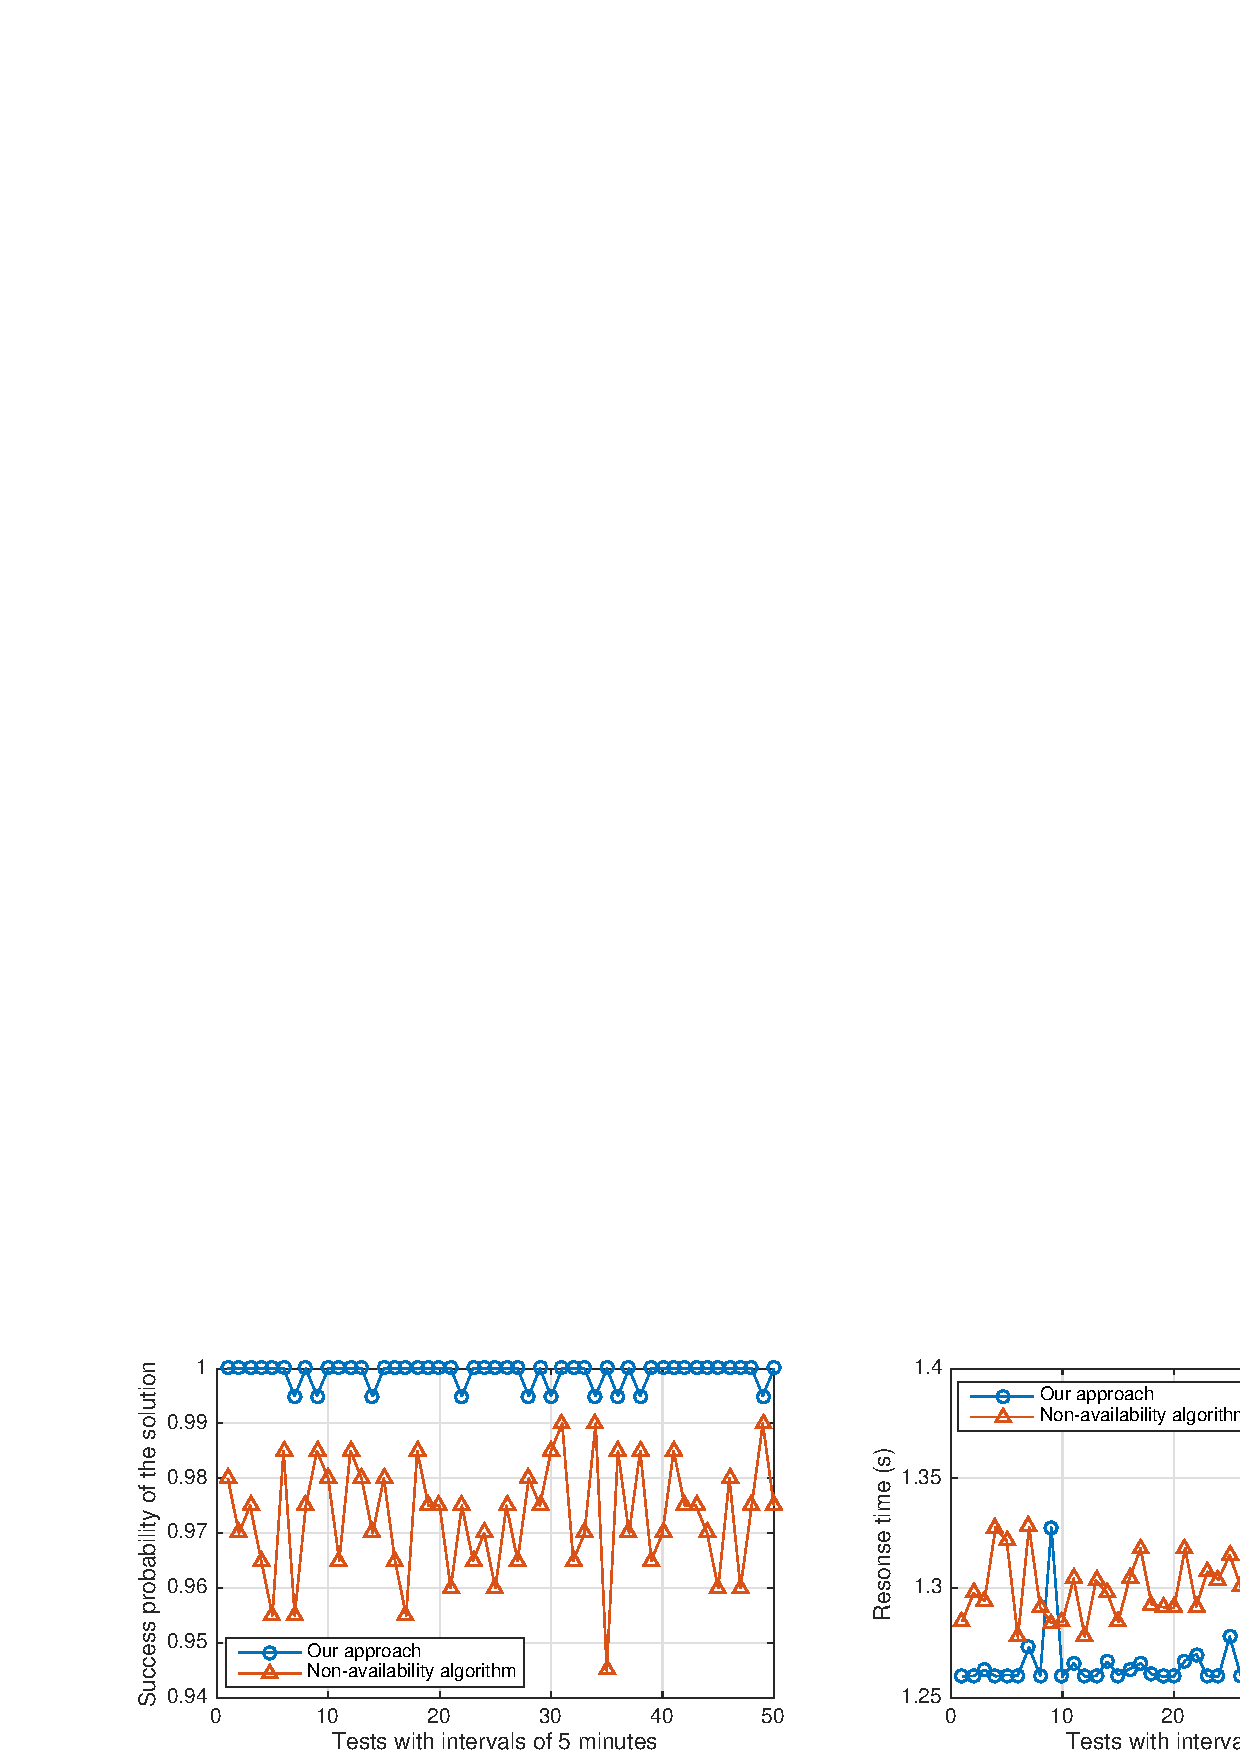
\includegraphics[width=3.2in]{./img/Task-6.pdf}
\caption{Case I}
\label{Task-6}
\end{figure}


\begin{figure}[!t]
\centering
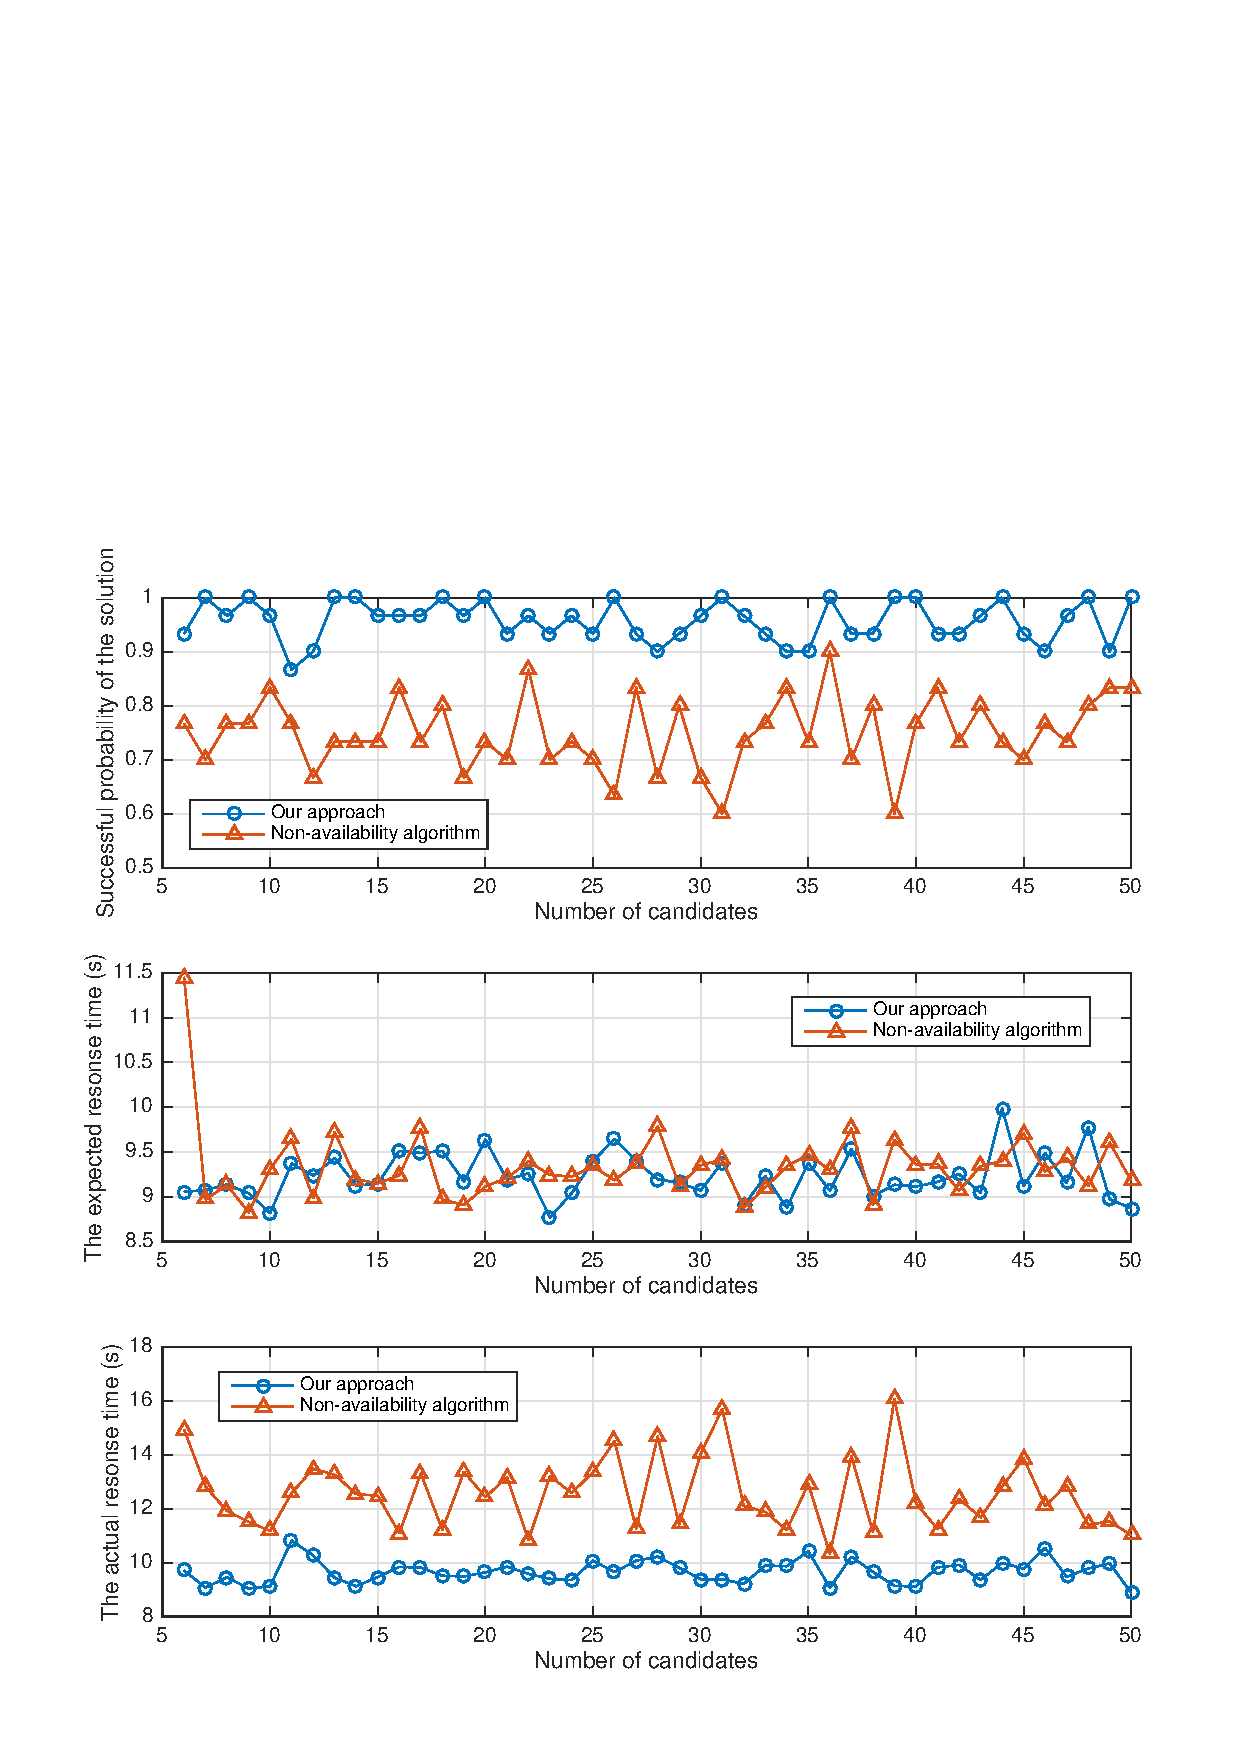
\includegraphics[width=3.2in]{./img/Task-12.pdf}
\caption{Case II}
\label{Task-12}
\end{figure}

\begin{figure}[!t]
\centering
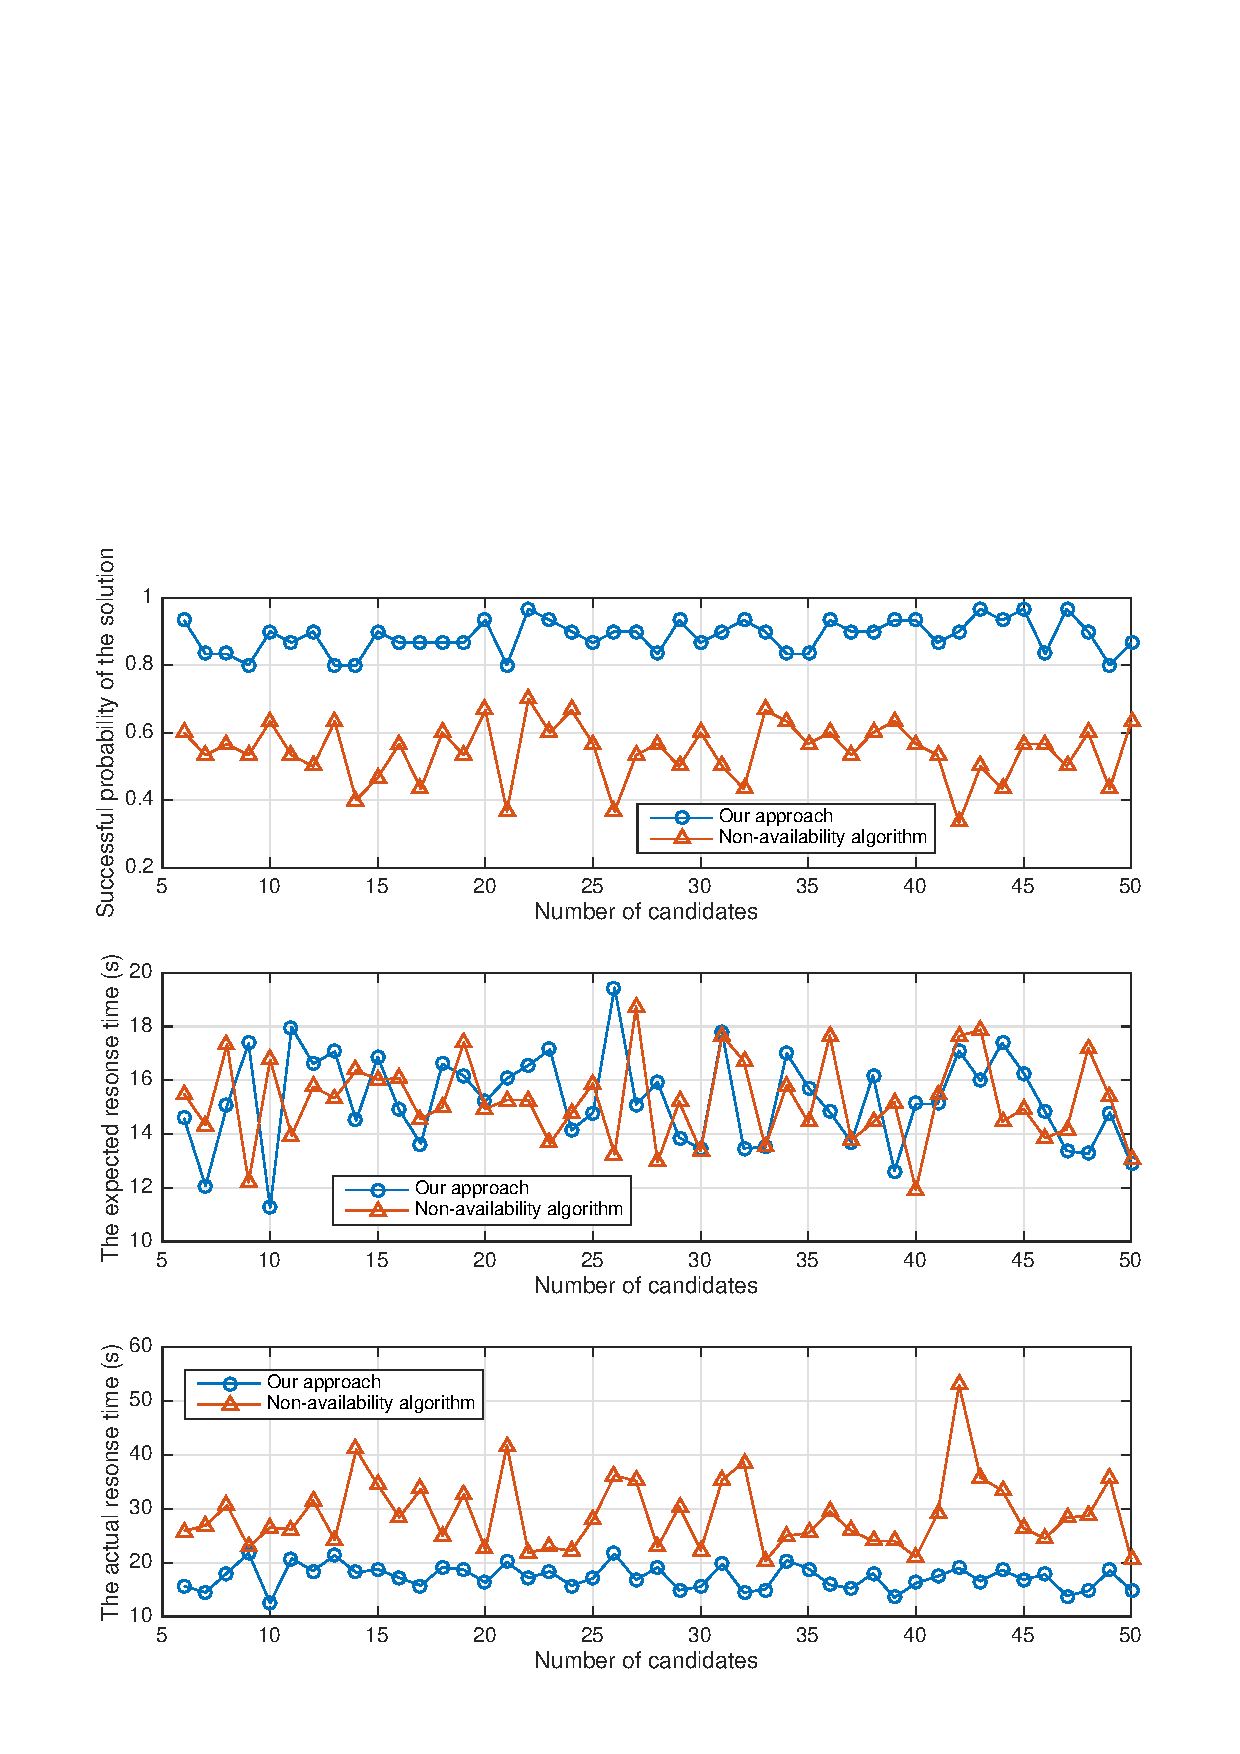
\includegraphics[width=3.2in]{./img/Task-24.pdf}
\caption{Case III}
\label{Task-24}
\end{figure}

As shown by Fig. 7(a), Fig. 8(a) and Fig. 9(a), our proposed method achieves higher success probability (by almost 100% 
for Case I, average 95% 
for Case II, and average 90% 
for Case III). From Fig. 7(b), Fig. 8(b) and Fig. 9(b) we can see, the solutions made by traditional mobile service composition approach which doesn't consider mobile service availability some times perform better than our method (especially in Case I). That is because our method consider both response time and service availability as optimization Object and in most of time our method can get the same performance as their approach. But in real mobile environment, low success probability means more time cost. A successful service composition response time is shown in Fig. 7(c), Fig. 8(c) and Fig. 9(c), it indicates that our method perform better in actual mobile environment.

Intuitively, the disadvantage of a non-availability approach lies in that it ignores mobility characteristic of mobile users. It therefore tends to choose the best provider who's QoS data is outstanding but will be not available in few second.


% \subsection{Optimality Evaluation}
% To verify the the capability of finding the optimal mobile service composition of our algorithms, we compare IKH with the basic GA algorithm, basic PSO algorithm and a brute-force algorithm.

% \textbf{Algorithm 1:} Improved Krill-herd mobile service composition algorithm (IKH) which described in Section 4.

% \textbf{Algorithm 2:} A basic GA which uses two-point crossover and uniform mutation.

% \textbf{Algorithm 3:} A basic PSO.

% \textbf{Algorithm 4:} A brute-force algorithm that traverses all feasible composition to find the optimal solution.

% To evaluate the optimality of above algorithms, we tune the parameters of each algorithm to achieve its best performance. The most suitable parameters are shown in Table 6.

% \begin{table}[!t]
% \renewcommand{\arraystretch}{1.3}
% \caption{Parameters setting for different algorithms}
% \label{table_example}
% \centering
% \begin{tabular}{cc}
% \hline
% \bfseries Algorithms & \bfseries Parameter Setting \\
% \hline
% GA  & crossover rate = 0.7; mutate rate = 0.3 \\
% PSO & inertia weight = 0.8; c1 = 2.0; c2 = 2.0 \\
% \hline
% \end{tabular}
% \end{table}

% \begin{figure*}[!t]
% \centering
% \subfloat[]{
% \includegraphics[width=2in]{./img/Opt-Iterations.pdf} 
% \label{PS}}
% \hfil
% \subfloat[]{
% \includegraphics[width=2in]{./img/Opt-Tasks.pdf} 
% \label{MI}}
% \hfil
% \subfloat[]{
% \includegraphics[width=2in]{./img/Opt-Candidates.pdf} 
% \label{CR}}

% \caption{Optimality evaluation.} \label{fig_sim}
% \end{figure*}

% The result in Fig. 7(a) shows that, as expected, the brute-force algorithm leads to the best performance with the highest QoS utility value. The basic PSO algorithm has the worst performance with the lowest QoS utility values. Both IKH and Ga can find over 95\% optimal composition before 30 iterations and IKH performs little better than the basic GA algorithm. 
% Fig. 7(a) and Fig. 7(b) shows that with the increasement of task number and service candidate number, our approach performs better than other algorithms.
% Although GA performs closely to IHK, IHK's superiority is it runs more faster than GA, in next subsection we will evaluate the scalability of above four algorithms.


% \subsection{Scalability Evaluation}
% In this experiment, we compared the run time of IKH with the other algorithms to evaluate the scalability of our algorithm.

% \begin{figure*}[!t]
% \centering
% \subfloat[Case I]{
% 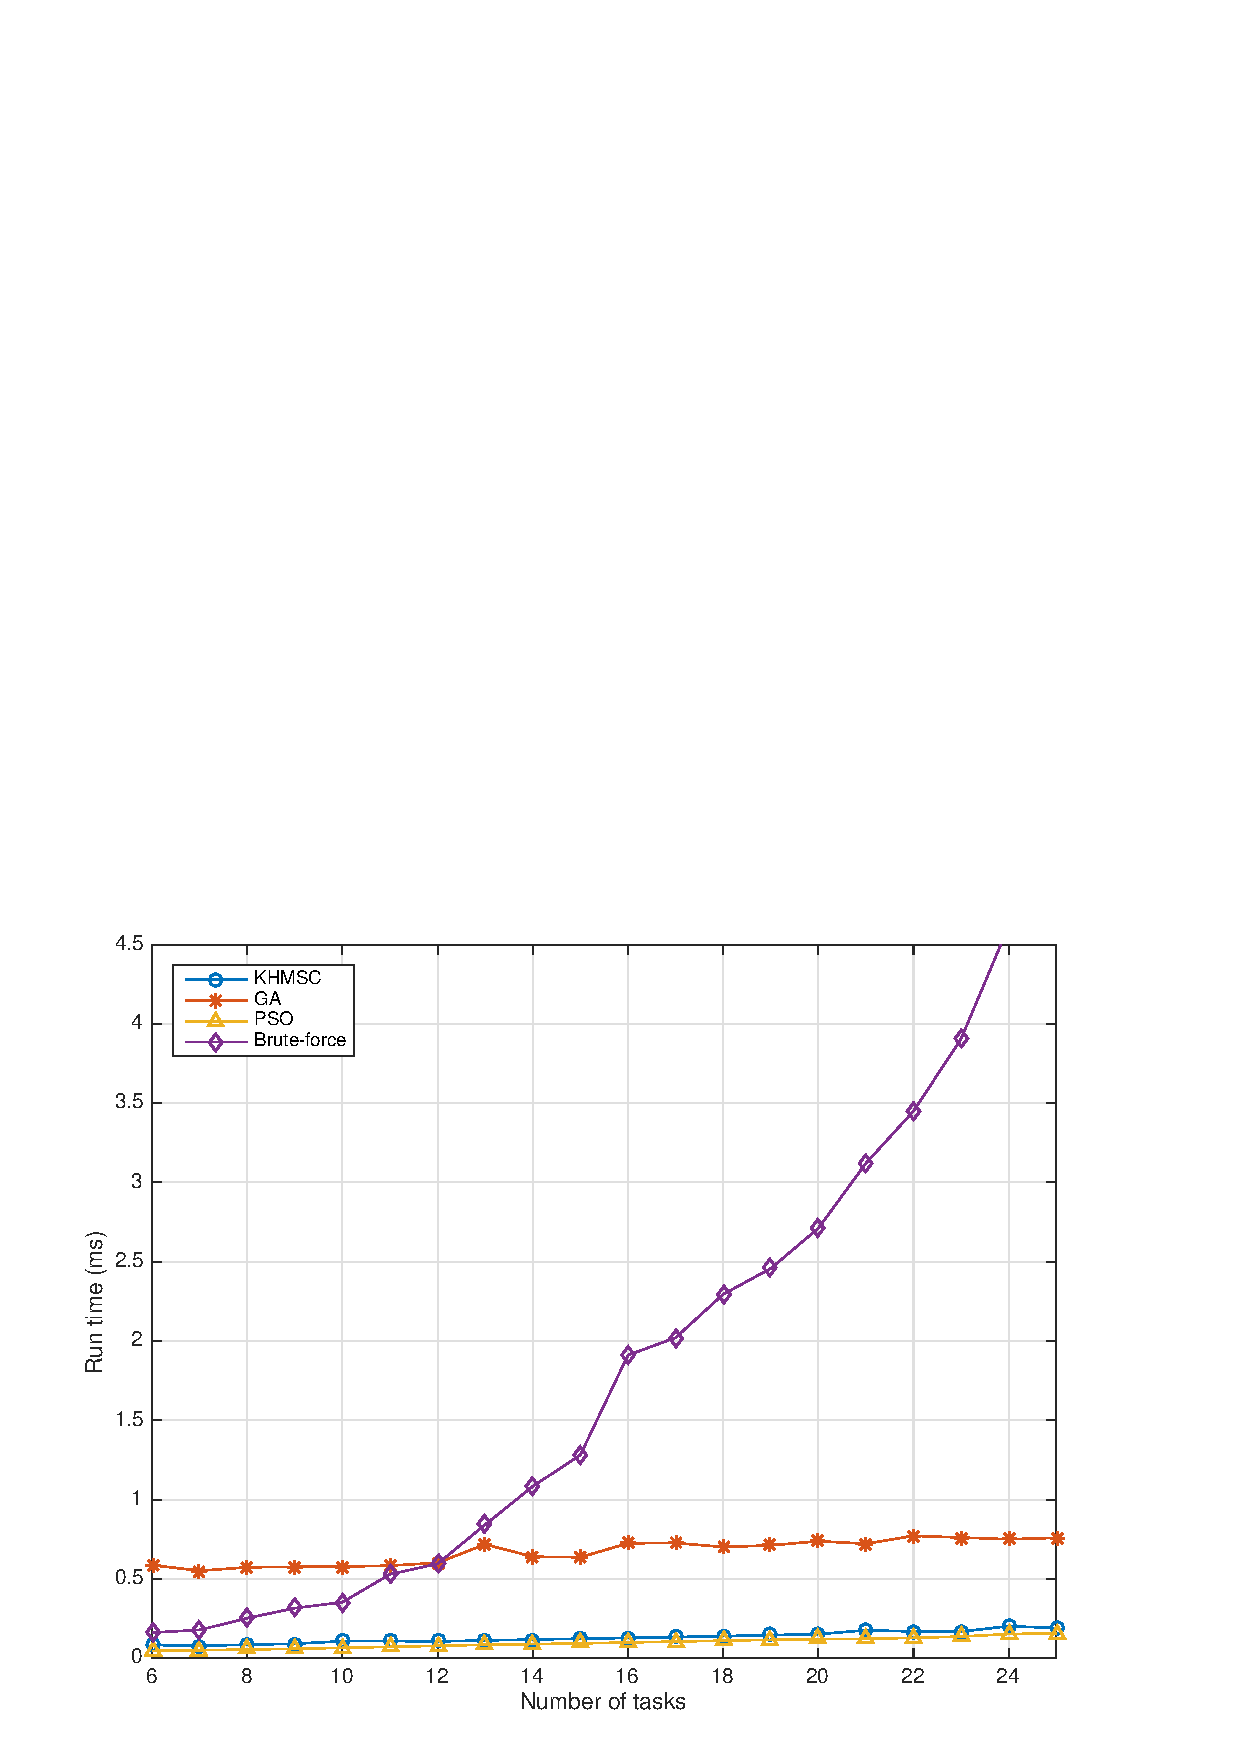
\includegraphics[width=3in]{./img/Sca-Tasks.pdf} 
% \label{Tasks}}
% \hfil
% \subfloat[Case II]{
% 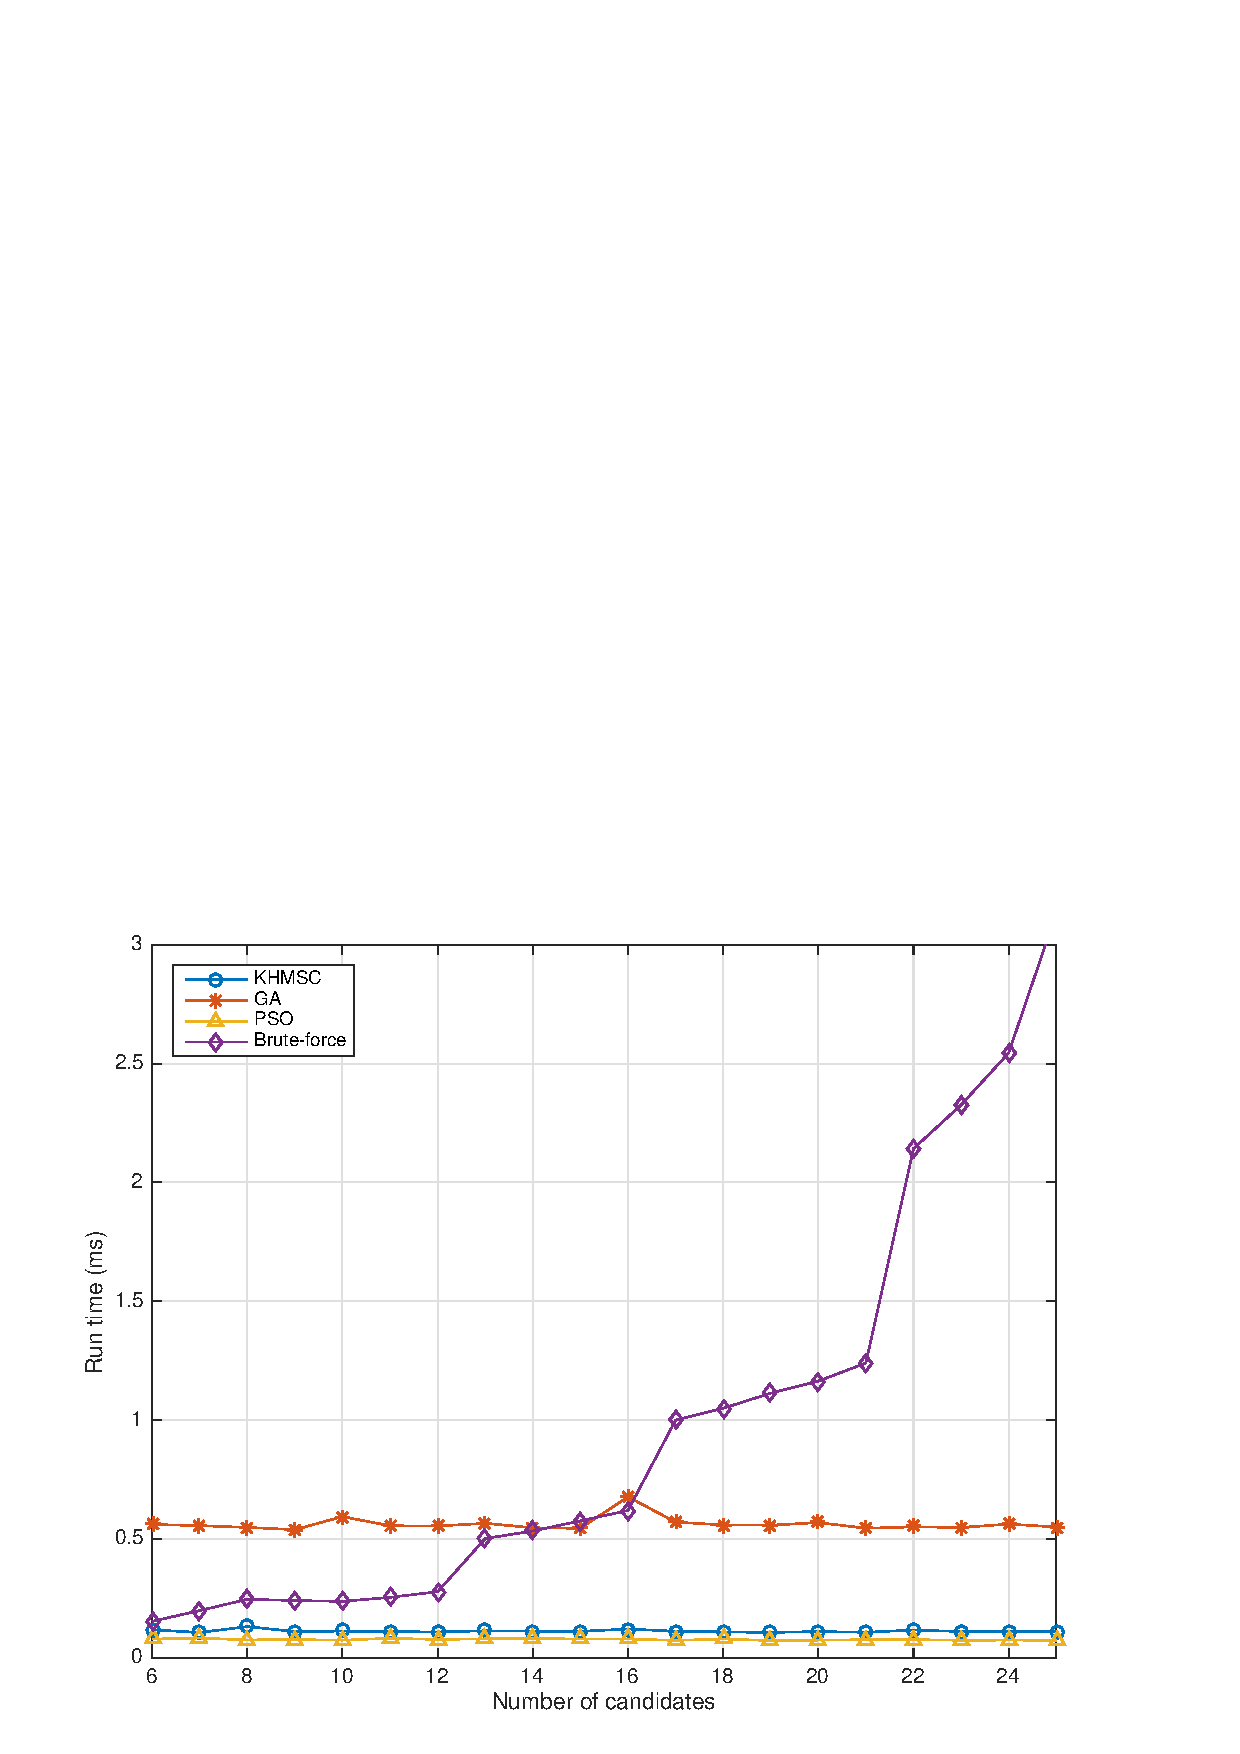
\includegraphics[width=3in]{./img/Sca-Candidates.pdf} 
% \label{Candidates}}

% \caption{Scalability evaluation.} \label{fig_sim}
% \end{figure*}

% In order to evaluate the impact of task number on the execution time of our algorithm, The task number is varied from 6 to 25. For each task number, the simulation is repeated 50 times, and the average performance was recorded as the result. We observe from Fig. 8(a) that with the increasement of task number, the run time of brute-force method is almost exponential to the problem size, while the run time of other three meta-heuristic algorithms (IKH, GA, PSO) are increases almost linearly with tasks increasing. In mobile environment, due to the dynamic movement and limited of computing resources, algorithm must meet the requirement of finding feasible composition within a short time. Therefore, although brute-force can obtain the optimal result, it is not suitable to the problem due to its poor scalability. 

% We also evaluate the impact of candidate services per task, In this experiment, we vary candidate service number from 6 to 25. As shown in Fig. 8(b), the number of candidate services does not affect the execution time of the three meta-heuristic algorithms, because in the initialization step, the scale of the algorithm is determined, and it is only affected by the algorithm parameters. Similarly, brute-force method is also exponential to the problem size. 

% Among all the algorithms, PSO has the lowest run time, then IKH, finally GA. But PSO's poor optimality makes it unsuitable for this problem, IKH runs almost five times faster than GA. Based on the experimental results, we can conclude that IKH maintains acceptable performance (optimality and scalability) with large data sets for both tasks and candidates.


\section{CONCLUSIONS AND FURTHER STUDIES}
In this paper, we propose a comprehensive framework for optimal mobile service compositing on mobile environment. We present a mobile service opportunistic network model (MSON) that fully integrates human mobility behavior factors for mobile service provisioning and introduce a QoS model for mobile service composition. Then we formulate the mobile service composition over MSON problem as an optimal problem to maximize the quality of service composition, propose a Krill-herd based algorithm to solve it, and a case study based on real-world opportunistic network and some well-known web service dataset show that our proposed approach outperforms current standard composition methods in mobile environments.

We plan to consider the following topics for future work: 1) Some prediction methods (e.g., hidden Markov model and neural networks) can be used to predict user future's movement to formulate a better user mobility model; 2) more QoS metrics (e.g., service price and service reputation) are supposed to be analyzed and blends into our QoS model; 3) this work doesn't consider Service-Level-Agreement (SLA) constrains. We intend to consider SLA constraints and introduce corresponding algorithms to generate better composition.

​		
​	

\bibliography{mybibtex}
\bibliographystyle{IEEEtran}

\end{document}






